\documentclass[letterpaper, 10pt, onecolumn, draftclsnofoot]{IEEEtran}

\usepackage[utf8]{inputenc}
\usepackage{listings}
\usepackage{geometry}
\usepackage{float}
\usepackage{enumerate}
\lstset{breaklines=true}
\geometry{margin=0.75in}
\usepackage{setspace}
\singlespacing
\usepackage{section}[placeins]
\usepackage{url}
\usepackage{array}
\usepackage{graphicx}
\usepackage{tabu}
\graphicspath{{./}}
\usepackage{booktabs}% http://ctan.org/pkg/booktabs
\newcommand{\tabitem}{\textbullet~~}

\renewcommand\thesection{\arabic{section}}
\renewcommand\thesubsection{\arabic{section}.\arabic{subsection}}
\renewcommand\thesubsubsection{\arabic{section}.\arabic{subsection}.\arabic{subsubsection}}

\usepackage[parfill]{parskip}

\begin{document}

% SECTION TITLE
\title{
    \Large{\textbf{AR Sandbox for Construction Planning \\
                   Traffic Simulation Feature Update}} \\
    \small{System Requirements Specification Document} \\
    \vspace{15pt}
    \large{Prepared for Dr. Joseph Louis \\
    Oregon State University \\
    School of Civil and Construction Engineering \\
    \today}
    }

\author{Team Augmented Construction Education \\
        McKenzie~Gray,~Jonah~Spencer,~and~Adam~Sunderman}
        
\maketitle
\vspace{100pt}
\begin{center}
\begin{tabular}{@{}p{.5in}p{4in}@{}}
Approved: & \hrulefill \\
& \hspace{10em} \\
Date: & \hrulefill \\
& \hspace{10em} \\
& Joseph Louis, Ph.D.\\
& Assistant Professor of Civil and Construction Engineering \\
& Oregon State University \\
\end{tabular}
\end{center}
\vspace{100pt}
%SECTION ABSTRACT
\begin{abstract}
    The following document describes the system requirement for a proposed upgrade to a currently operating Augmented Reality Sandbox located at Oregon State University. Currently the AR Sandbox has the ability to display topographic information and segments of roads within the sandbox that are used in construction planning. The upgrade will refine the functionality and usability of previously built modules as well as add new functionality in the form of traffic simulation and interactive object placement.
\end{abstract}
\newpage

\tableofcontents
\newpage

% SECTION CHANGELOG
\section{\textbf{Change Log}}
\renewcommand{\arraystretch}{4}
\begin{center}
    \begin{tabular}{|p{4cm}|p{6cm}|p{6cm}|}
        \hline
        \centering \textbf{\large Section} & \centering \textbf{\large Original} & \centering \textbf{\large New} \tabularnewline
        \hline
        \centering \textbf{System Functions} & 
        \tabitem Defined a requirement for "Design Mode", which would be used to create road networks. \newline & 
        \tabitem Removed "Design Mode" and moved the requirements to "Traffic Simulation Mode". \\
        \hline
        \centering \textbf{Functional Requirements} & 
        \tabitem Included a requirement for perspective view, but no requirement for microscopic view. \newline 
        \tabitem Specified use of markers for scene creation. \newline 
        \tabitem Save and load terrains in the old AR Sandbox. \newline
        \tabitem Sight lines for vehicles in simulations. \newline &
        \tabitem Clarified requirements for "Traffic Simulation". \newline
        \tabitem Removed requirement for perspective view from "Traffic Simulation". \newline 
        \tabitem Added requirement for microscopic view to "Traffic Simulation". \newline 
        \tabitem Made marker requirements more broad/generic. \newline
        \tabitem Moved terrain save/load to stretch goals. \newline
        \tabitem Moved sight lines to stretch goals. \\
        \hline
        \centering \textbf{Usability Requirements} & 
        \tabitem Specified use of markers for scene creation. \newline & 
        \tabitem Made marker requirements more broad/generic. \\
        \hline
        \centering \textbf{System Operations} & 
        \tabitem Specified use of markers for scene creation. \newline & 
        \tabitem Made marker requirements more broad/generic. \\
        \hline
    \end{tabular}
\end{center}
\newpage

% SECTION INTRODUCTION
\section{\textbf{Introduction}}
    \subsection{\textbf{System Purpose}}
        The purpose of the AR Sandbox is mainly educational and meant as a means to visualize large scale construction projects. The AR Sandbox offers a new and unique way for students to visualize the topics they learn in class with real-time feedback supported by various augmented reality modules.
    
    \subsection{\textbf{System Scope}}
        The system currently contains several modules for doing various tasks within the AR Sandbox. These modules include a cut-and-fill mode for calculating earth moving requirements for large transportation projects, a topographical mode for displaying current sand height information within the sandbox, and a design mode for projecting and editing sections of roadway.
        
        The proposed upgrade will add modules giving users the ability to create full road networks and place scene items without the need for a keyboard or mouse. These scenes will create the imagery projected in the AR Sandbox and form an digital infrastructure that traffic simulations can be ran on.
    
    \subsection{\textbf{System Overview}}
        \subsubsection{\textbf{System Context}}
        See Appendix A for a diagram of the AR Sandbox. 
        
        \subsubsection{\textbf{System Functions}}
        The AR Sandbox should have the following functionality.
        \begin{enumerate}[\label={}]
            \item {\textbf{\emph{Topographical Projections:}} The AR Sandbox should project a digital representation of the sandboxes current topography. This should be represented as a color gradient from red (high) to blue (low) with contour lines that join points of equal height. This is currently partially complete.}
            
            \item {\textbf{\emph{Object and Road Projections:}} The AR Sandbox should project a digital representation of user created road networks and the objects around them that form a scene.}
            
            \item {\textbf{\emph{Object Recognition:}} The AR Sandbox should have a way to convert real world objects that a user places in the sandbox into the appropriate model for a scene.}
            
            \item {\textbf{\emph{Cut and Fill Mode:}} The AR Sandbox should project cut and fill requirements for road segments while in design mode. This is currently complete, but needs adjustments.}

            \item {\textbf{\emph{Traffic Simulation Mode:}} The AR Sandbox should allow users to create scenes with road networks for the purpose of visualizing traffic simulations. Scene items should include streets, buildings and traffic lighting but could be any arbitrary item. Traffic simulations should run in real-time on a created road network and should be interactive to allow for changes at run time.}
        \end{enumerate}
        
        \subsubsection{\textbf{User Characteristics}}
        The users of the AR Sandbox will be professors and students at Oregon State University's School of Civil and Construction Engineering. Students and instructors that deal with transportation engineering should be a major focus of the new module but not the system as whole. Instructors should be able to use the AR Sandbox for in-class demonstrations while students should have the ability to explore class topics. 
        
    \subsection{\textbf{Definitions}}
    \begin{enumerate}[\label={}]
        \item {\textbf{AR Sandbox:} Augmented reality sandbox. A physical sandbox with a depth sensor and projector that displays graphics on the sand, such as roadways and ground topography.}
        
        \item {\textbf{Augmented Reality:} A way of mixing computer images with the user’s vision. This refers to the graphics displayed over the sand. When a user manipulates the sand, the graphics displayed on the sand will change.} 
        
        \item {\textbf{CPU:} Central Processing Unit. The computer component that handles general processing instructions.}
         
        \item {\textbf{Cut and Fill:} Excavation, amounts of earth (dirt, rock, etc.) that must be moved, removed or brought into a location in order to create an acceptable terrain for a project.}
        
        \item {\textbf{Depth Sensor:} A digital imaging device which uses a gray-scale image to represent the distance from the sensor to the nearest surface.}
        
        \item{\textbf{Game Engine:} A program or set of programs that help game developers create games. A game engine helps manage various game features and tasks such as graphics rendering, input devices, audio, physics, scripting and networking.}
        
        \item {\textbf{GPU:} Graphics Processing Unit. A computer component that handles graphics processing.}
        
        \item {\textbf{Markers:} Markers are physical objects that a user can place and move within in the AR Sandbox. Markers represent a real-world object that a user would like to add to the current AR Sandbox scene such as a building or road. A marker 'signals' the system to project the specified objects image at the markers exact location.}       
        
        \item {\textbf{Projection:} The image cast on the sand’s surface by the projector.}
        
        \item{\textbf{Shader:} A specialty program for graphics that tells the computer how to render (display) each pixel in an image.}
        
        \item {\textbf{Topography:} The surface elevation features of the sand in the AR Sandbox at any given time. Measured from all points in the AR Sandbox and projected as a color gradient from red to blue that covers the sands surface.}
    \end{enumerate}
    
%SECTION REFERENCES
\section{\textbf{References}}
    \begin{enumerate}[\label={}]         
        \item{Original UC Davis AR Sandbox: \url{https://arsandbox.ucdavis.edu/}}
        \item{Original OSU Design Documents: \url{https://github.com/soltesza/AR-Sandbox-for-Construction-Planning}}
    \end{enumerate}

%SECTION REQUIREMENTS
\section{\textbf{System Requirements}}
    \subsection{\textbf{Functional Requirements}}
    \begin{enumerate}[\label={}]
    
        \item{\textbf{Traffic Simulation:} The system will be able to perform traffic simulations with pre-loaded and user-built road maps. This simulation will need to be realistic enough to be used in a classroom setting. Traffic simulations should be able to be viewed mesoscopically, where colored sections of roadway indicate how well traffic is moving, or microscopically, where the behavior of individual cars can be observed.}
        
        \item{\textbf{Sight-line Visualization:} The system will be able to calculate the AR Sandbox's current terrain features to determine passing zones for various stretches of roads. Elevated terrain around roadway sections will be used to determine visibility at these locations which will then be projected on the road as a cone of vision. This feature is still in production but was moved to a stretch goal for the development team.}
        
        \item{\textbf{Terrain Capture:} The system will be able to save a terrain mesh of a current terrain to be used later in the AR Sandbox. This feature was also moved to a stretch goal. Terrains are currently saving but cannot load until a new shader is written.}
        
        \item{\textbf{Mass-Haul Simulation:} The system will be able to create a mass-haul diagram comparing the current terrain and a pre-defined (possibly previously captured) terrain. This diagram will show where sand needs to be removed and where sand needs to be added to make sand in the AR Sandbox match the terrain model.}
        
        \item{\textbf{Markers:} The system will have a marker system which will identify an object type that a user is attempting to place in the AR Sandbox. Markers will be unique physical objects that a user will introduce and manipulate within the AR Sandbox. These markers will be the main user interface for traffic simulations, mode selection, and general interactions.}
        
        \item{\textbf{Computer Vision / Object Recognition:} The system must be able to identify various marker types that a user will place in the AR Sandbox in order to interact with the system in various ways.}
        
        \item{\textbf{Model Library:} The system must have a sufficiently large collection of various pre-built 3D models. These models will be displayed in the sandbox at a marker location and match the marker type. The models should include buildings, street lights, signs, various roadway features, and urban elements.}
        
        \item{\textbf{Game Engine:} The system must utilize a game engine to handle graphics, user input, and general run time logic. The choice has been previously made to use Unity Game Engine.}
        
    \end{enumerate}
        
    \subsection{\textbf{Usability Requirements}}
    The system must be able to allow users to create scenes and interact with simulations with minimal use of a keyboard and mouse. Markers should replace mouse and keyboard interaction wherever possible.
        
    \subsection{\textbf{Performance Requirements}}
    The system will use computer graphics drawn in real time and therefor should be sufficiently capable to run the required code. The system must have a powerful GPU for the graphics shaders required in topographic projections and the rendering of user created scenes. The system must also have a powerful CPU for handling simulation logic in addition to general processing tasks. 
        
    \subsection{\textbf{System Interface}}
    Markers should be available for multiple object types and be easily distinguishable from each other. Markers may or may not remain in a scene after being identified by the system and added to the scene. Calibration and various system setup procedures may still make use of keyboard and mouse input.
    
    \subsection{\textbf{System Operations}}
    \begin{enumerate}[\label={}]         
        \item{\textbf{Scene Creation:} The system must have a game engine to handle graphics, user input, and general run time logic.}
        
        \item{\textbf{Ease of Use:} The system must allow for creation and interaction of traffic simulations with minimal use of a keyboard and mouse. Markers should replace mouse and keyboard input wherever possible.}
        
        \item{\textbf{Maintainability:} The system must be easily modifiable and extensible so next years students can continue development. This should be accomplished by adding new modules and levels to the current game logic.}
    \end{enumerate}
    
    \subsection{\textbf{Information Management}}
    The system must have a database or similar data storage option for storing information related to markers. As a marker is read by the system the markers type will be translated to the proper 3D model for display in the AR Sandbox. The model itself will be stored along with any model data that can be used in traffic simulations. 
    
%SECTION VERIFICATION
\section{Verification}
    \subsection{\textbf{Functional Requirements}}
        \begin{enumerate}[\label={}]
           \item{\textbf{Traffic Simulation:} The traffic simulation must represent realistic traffic patterns that are visible in the scene. Interacting with the system using markers must result in a reasonably realistic change in the simulation.}
        
            \item{\textbf{Sight-line Visualization:} The system must determine passing zones for various stretches of arbitrary road. Moved to stretch goals.}
            
            \item{\textbf{Terrain Capture:} The system must be able to save and load a terrain mesh. Partially implemented, moved to stretch goals.}
            
            \item{\textbf{Mass-Haul Simulation:} The system must provide accurate, deterministic data.}
            
            \item{\textbf{Markers:} Users must be able to interact with physical markers in the sandbox that interact with the virtual environment. This interaction must not require any mouse or keyboard input.}
            
            \item{\textbf{Computer Vision / Object Recognition:} The system must be able to recognize a predefined library of markers and update the simulation in real time.}
            
            \item{\textbf{Model Library:}  Models must have simulation data in addition to the objects physical data.}
        
            \item{\textbf{Game Engine:} The engine must use the data from the depth sensor and object recognition software to render the scene through the projector. The scene must update in real time according to user interaction via markers.}
        \end{enumerate}
    
    \subsection{\textbf{Usability Requirements}}
    Interaction with the AR sandbox must include minimal interaction with the keyboard and mouse. These input methods may be necessary for system setup and calibration, but further interaction must be entirely sand- and marker-based.
    
    \subsection{\textbf{Performance Requirements}}
    The system must be able to run simulations without any noticeable slowdown or skipping. User interaction must register in the projected scene in real time with minimal latency (no more than a few seconds).
    
    \subsection{\textbf{System Interface}}
    Various markers must be available for use in the sandbox. It must be possible for users to place markers in the sandbox and doing so must result in a change in the scene and the simulation.

    \subsection{\textbf{System Operations:}}
        \begin{enumerate}[\label={}]
        \item{\textbf{Cut \& Fill Mode} The cut \& fill mode is complete but requires improvement to meet the Usability Requirements above.}
        
        \item{\textbf{Design Mode:} Users must be able to create scenes in the sandbox using markers. Scenes must include, at minimum, roads, buildings, and traffic lights. The user must be able to save a scene made in design mode and load that scene in either design mode or traffic simulation mode. Design mode conflicts with a previously named mode in the original AR Sandbox. As a result Design Mode and Traffic Simulation Mode (below) are now considered as parts of the same mode.}
        
        \item{\textbf{Traffic Simulation Mode:} Users must be able to load scenes created in design mode and visualize a traffic simulation in the scene. The simulation must change according to placement and location of markers in the scene.}
    \end{enumerate}
    
    \subsection{\textbf{Information Management}}
    Tests must be ran to verify that data is being saved and loaded as expected. These tests should cover both simulation and marker/model data. That is, a marker should produce the proper model and that model should have the correct data to represent the real world object in simulations.  
    
\newpage
%SECTION APPENDICES
\appendices
    \section{AR Sandbox Diagram}
        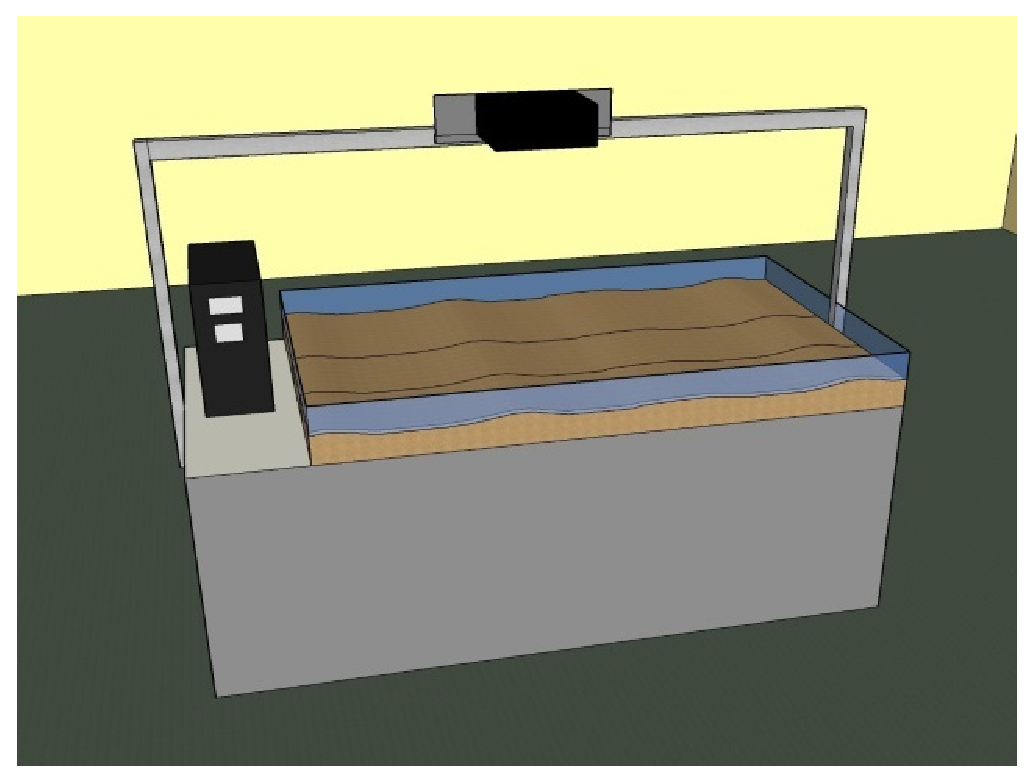
\includegraphics{ARSandbox.eps}
    \section{AR Sandbox Block Diagram}
        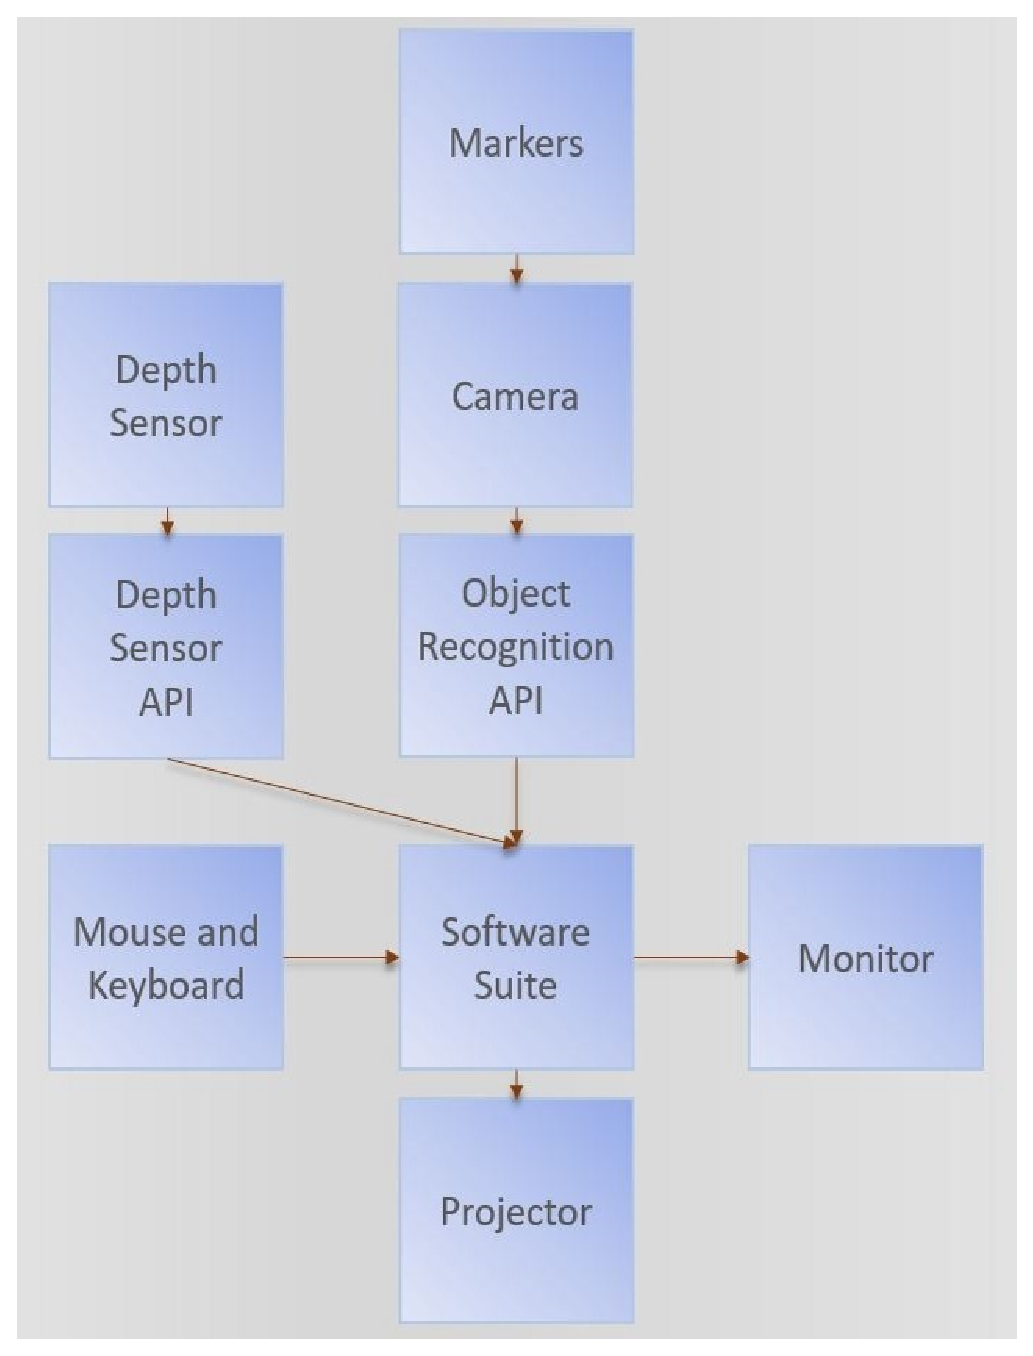
\includegraphics{BlockDiagram.eps}
    \section{Project Timeline}
        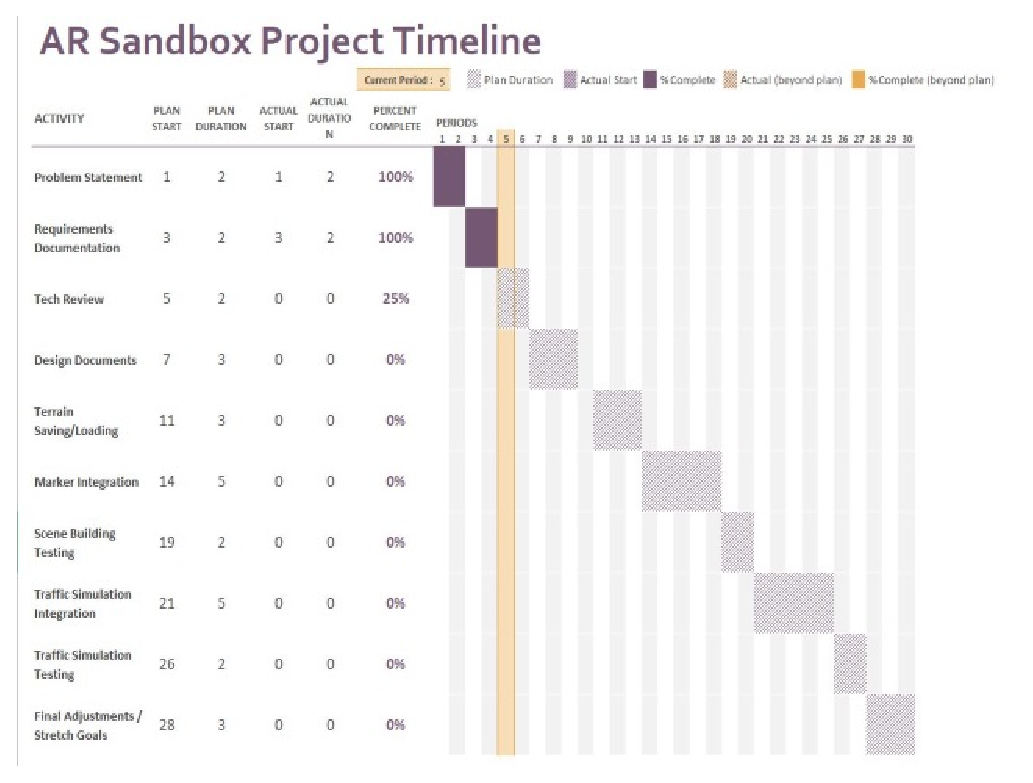
\includegraphics{Gantt.eps}

\newpage
%SECTION ACKNOWLEDGMENT
\section
*{Acknowledgment}
A Special thanks to Raja Petroff, Andrew Soltesz and Mark Sprouse (Team Sandy) for developing the first version of OSU's AR Sandbox, and UC Davis for inspiring all AR Sandbox projects across the country.  

\end{document}